\begin{frame}
  \begin{columns}
    \begin{column}{0.45\textwidth}
      \vspace{-1em}
      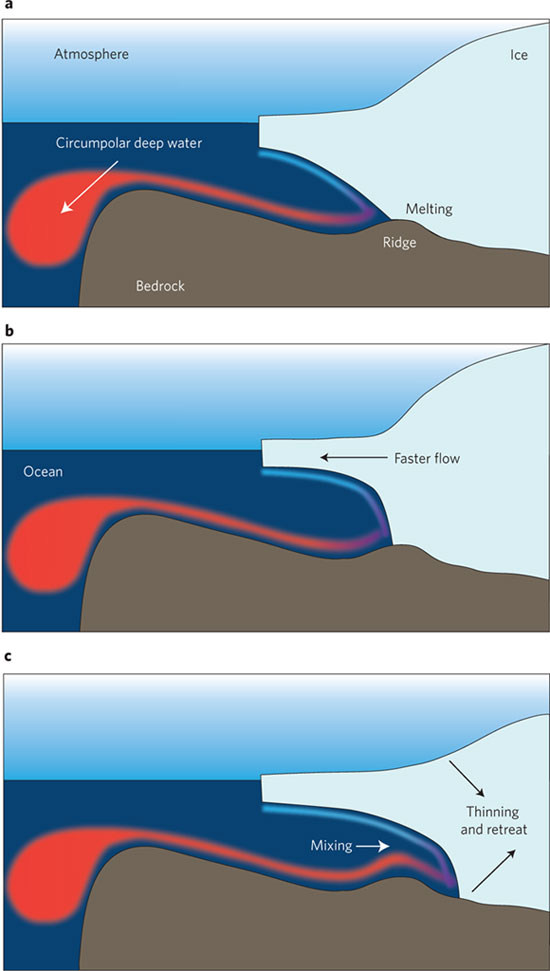
\includegraphics[width=\textwidth]{figures/GroundingLine/SchoofNature2010} \\
\footnotesize{(Schoof 2010)}
    \end{column}
    \begin{column}{0.55\textwidth}
      {\large \color{blue}{$y^+$ underneath an ice shelf}}
    \begin{itemize}
    \item Order of magnitude dimensions: length \unit{100}{\meter},       speed \unit{10}{\centi\meter\per\second}
    \item Viscous boundary layer: $y^+ \in \bigO(1) \implies       \unit{1}{\milli\meter}$ grid
    \item No-slip boundary conditions requires \emph{resolution} of this       layer % (wall resolution)
    \item Otherwise we need nonlinear slip
      \begin{itemize} \item still usually $y^+ \in \bigO(100)$       \end{itemize}
    \item Estimates come from validation (lab experiments) with heat       transfer in industrial and aerospace applications
    \item Thermohaline boundary layer: \unit{\text{1--10}}{\meter}
    \item Boundary layer equations require solution of a Riemann problem
    %\item Is simulation of this process plausible without boundary-fitted meshes?
    \end{itemize}
   \end{column}
  \end{columns}
\end{frame}

% \begin{frame}{$y^+$ underneath an ice shelf}
%   \begin{itemize}
%   \item Order of magnitude dimensions:
%     length \unit{100}{\meter}, speed \unit{10}{\centi\meter\per\second}
%   \item Viscous boundary layer: $y^+ \in \bigO(1) \implies % \unit{1}{\milli\meter}$ grid spacing
%   \item No-slip boundary conditions requires \emph{resolution} of this % layer % (wall resolution)
%   \item Otherwise we need nonlinear slip conditions
%     \begin{itemize} \item still usually $y^+ \in \bigO(100)$ % \end{itemize}
%   \item Estimates come from validation (lab experiments) with heat
%     transfer in industrial and aerospace applications
%   \item Thermohaline boundary layer is \unit{\text{1--10}}{\meter}
%   \item Boundary layer equations require solution of a Riemann problem
%   \item Is simulation of this process plausible without \\
%     boundary-fitted meshes?
%   \end{itemize}
% \end{frame}

\begin{frame}{LES+RANS with wall modeling}
  \begin{itemize}
  \item State of the art for high-Reynolds separating flows
  \item Subshelf circulation separates when it reaches neutral buoyancy \\ (this is a crucial limiting process)
  \item Is it possible to accurately predict heat transfer, separation, and overturning with $y^+ \in \bigO(10^5)$?
  \end{itemize}
  \begin{quotation}
    %Also, it
    It has been repeatedly observed, especially at high Reynolds     numbers and coarse grids and with the interface location being around     $y^+ = \bigO(100-200)$, that the high turbulent viscosity generated by     the turbulunce model in the inner region extends, as subgrid-scale     viscosity, deeply into the outer LES region, causing severe damping in     the resolved motion and a misrepresentation of the resolved structure as     well as the time-mean properties.
  \end{quotation}
  (Tessicini, Li, Leschziner, \emph{Simulation of Separation from Curved Surfaces with Combined LES and RANS Schemes}, 2007)
\end{frame}